\documentclass[A4,12pt, utf8]{article}
\usepackage{tikz}
\usepackage[
    backend=biber,
    style=authoryear-icomp,
    sortlocale=de_DE,
    natbib=true,
    url=false, 
    doi=true,
    eprint=false
]{biblatex}
\usepackage{listings}
\usepackage{xcolor}
\usepackage{hyperref}
\usepackage{pgf}
\usepackage{tikz}
\usetikzlibrary{arrows,automata}
\usepackage{todonotes}
\usepackage{dirtree}
\usepackage{pdflscape}
\usepackage{csquotes}
\MakeOuterQuote{"}


\newcommand{\tinytodo}[2][]
   {\todo[caption={#2}, size=\small, #1]{\renewcommand{\baselinestretch}{0.5}\selectfont#2\par}}

\colorlet{punct}{red!60!black}
\definecolor{background}{HTML}{EEEEEE}
\definecolor{delim}{RGB}{20,105,176}
\colorlet{numb}{magenta!60!black}

\lstdefinelanguage{json}{
    basicstyle=\normalfont\ttfamily,
    % numbers=left,
    % numberstyle=\scriptsize,
    % stepnumber=1,
    % numbersep=8pt,
    showstringspaces=false,
    breaklines=true,
    frame=lines,
    backgroundcolor=\color{background},
    literate=
     *{0}{{{\color{numb}0}}}{1}
      {1}{{{\color{numb}1}}}{1}
      {2}{{{\color{numb}2}}}{1}
      {3}{{{\color{numb}3}}}{1}
      {4}{{{\color{numb}4}}}{1}
      {5}{{{\color{numb}5}}}{1}
      {6}{{{\color{numb}6}}}{1}
      {7}{{{\color{numb}7}}}{1}
      {8}{{{\color{numb}8}}}{1}
      {9}{{{\color{numb}9}}}{1}
      {:}{{{\color{punct}{:}}}}{1}
      {,}{{{\color{punct}{,}}}}{1}
      {\{}{{{\color{delim}{\{}}}}{1}
      {\}}{{{\color{delim}{\}}}}}{1}
      {[}{{{\color{delim}{[}}}}{1}
      {]}{{{\color{delim}{]}}}}{1},
}
% \addbibresource{linked.bib}

\newcounter{treeline}

\newcommand{\treeroot}[1]{% Title
\node[above] at (0,0) {#1};%
\setcounter{treeline}{0}
}

\newcommand{\treeentry}[2]{% Title, Level
\draw[->] (#2-1,-\value{treeline}/2) -- (#2-1,-\value{treeline}/2-0.5) -- (#2+0.5,-\value{treeline}/2-0.5) node[right] {#1};
\stepcounter{treeline}
}

\newcommand{\altentry}[2]{% Title, Level
\draw[->] (#2-1,-\value{treeline}/2) -- (#2-1,-\value{treeline}/2-0.5) -- (#2+0.5,-\value{treeline}/2-0.5) node[right] {#1};
\foreach \x in {1,...,#2}
{   \draw (\x-1,-\value{treeline}/2) -- (\x-1,-\value{treeline}/2-0.5);
}
\stepcounter{treeline}
}


\title{emuLVC - Stucture of the angularjs app}
\author{Raphael Winkelmann}
\date{\today}
\begin{document}
  % \maketitle

\section{Schematic DB file structure on disc}

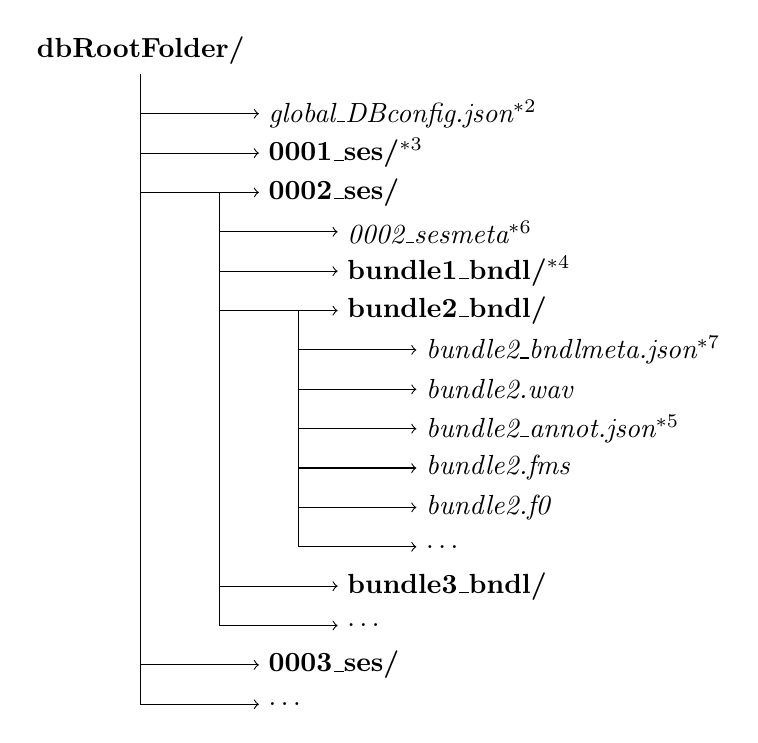
\begin{tikzpicture}
\treeroot{\textbf{dbRootFolder/}}
\altentry{\textit{global\_DBconfig.json$^{*2}$}}{1}
\altentry{\textbf{0001\_ses/$^{*3}$}}{1}
\altentry{\textbf{0002\_ses/}}{1}
\altentry{\textit{0002\_sesmeta$^{*6}$}}{2}
\altentry{\textbf{bundle1\_bndl/$^{*4}$}}{2}
\altentry{\textbf{bundle2\_bndl/}}{2}
\altentry{\textit{bundle2\_bndlmeta.json$^{*7}$}}{3}
\altentry{\textit{bundle2.wav}}{3}
\altentry{\textit{bundle2\_annot.json$^{*5}$}}{3}
\altentry{\textit{bundle2.fms}}{3}
\altentry{\textit{bundle2.f0}}{3}
\altentry{\dots}{3}
\altentry{\textbf{bundle3\_bndl/}}{2}
\altentry{\dots}{2}
\altentry{\textbf{0003\_ses/}}{1}
\altentry{\dots}{1}
\end{tikzpicture}


\begin{itemize}
  \item $^{*2}$: global config information file (similar to \textit{.tpl} file of old EMU). Specifies things like structure of hierarchy and possible perspectives to look at the DB (relevant for layout of labeler). \textit{\_DBconfig.json} is a fix suffix and the prefix should be the same as the database name field in the file itself.
  \item $^{*3}$: \textit{\_ses} is a fix suffix specifying the folder as being a session folder. Preceding this suffix can be anything as long it is unique on a session level (OS won't let you name two folders the same anyway...). If no session is required a dummy session is used called 0000\_ses.
  \item $^{*4}$: a bundle encapsulates what used to be known as an utterance in a folder. This includes signal files (\textit{wav, SSFF}) and the new annotation file (see $^{*5}$). Unknown file extensions are ignored. \textit{\_bndl} is a fix suffix specifying the folder as being a bundle folder.
  \item $^{*5}$: annotation file containing label and level information as well as hierarchical information (see listing 1). \textit{\_annot.json} is a fix suffix and the prefix should be the same as the bundle name.
  \item $^{*6}$: Optional session meta information file. Simple key-value json of the form \{"key1":"value1", "key2":"value2"\}
  \item $^{*7}$: Optional bundle meta information file. Simple key-value json of the form \{"key1":"value1", "key2":"value2"\}
\end{itemize}



%%%%%%%%%%%%%%%%%%%%%%%%%%%%%%%%%%%%%%
%%%%%%%%%%%%%%%%%%%%%%%%%%%%%%%%%%%%%%
%%%%%%%%%%%%%%%%%%%%%%%%%%%%%%%%%%%%%%
\section{File structure of json files}

The EMU-webApp supports several JSON file types for which individual schema are available (all of type:
\texttt{http://json-schema.org/draft-04/schema\#})

\section{Schema files}

There are two sets of schema files. The ones being used by the current live version of the web application 
(\url{http://ips-lmu.github.io/EMU-webApp/}) and the ones used by the current development version.
The two sets are usually quite similar if not identical as we try to keep the file definitions as
constant as possible.

The schema files used by the current live version are:

\todo[inline]{redo after schema cleanup}

\begin{itemize}
  \item \textbf{DBconfigFileSchema}: \href{https://github.com/IPS-LMU/EMU-webApp/blob/master/dist/schemaFiles/DBconfigFileSchema.json}{GitHub link}
  \item \textbf{annotationFileSchema}: \href{https://github.com/IPS-LMU/EMU-webApp/blob/master/dist/schemaFiles/annotationFileSchema.json}{GitHub link}
  \item \textbf{bundleSchema}: \href{https://github.com/IPS-LMU/EMU-webApp/blob/master/dist/schemaFiles/bundleSchema.json}{GitHub link}
  \item \textbf{bundleListSchema}: \href{https://github.com/IPS-LMU/EMU-webApp/blob/master/dist/schemaFiles/bundleListSchema.json}{GitHub link}
  \item \textbf{emuwebappConfigSchema}: \href{https://github.com/IPS-LMU/EMU-webApp/blob/master/dist/schemaFiles/emuwebappConfigSchema.json}{GitHub link}
  \item \textbf{emuwebappConfigSchema}: \href{https://github.com/IPS-LMU/EMU-webApp/blob/master/dist/schemaFiles/emuwebappConfigSchema.json}{GitHub link}
\end{itemize}

The schema files for the development version are:

\begin{itemize}
  \item \textbf{DBconfigFileSchema}: \href{https://github.com/IPS-LMU/EMU-webApp/blob/master/dist/schemaFiles/DBconfigFileSchema.json}{GitHub link}
  \item \textbf{annotationFileSchema}: \href{https://github.com/IPS-LMU/EMU-webApp/blob/master/dist/schemaFiles/annotationFileSchema.json}{GitHub link}
  \item \textbf{bundleSchema}: \href{https://github.com/IPS-LMU/EMU-webApp/blob/master/dist/schemaFiles/bundleSchema.json}{GitHub link}
  \item \textbf{bundleListSchema}: \href{https://github.com/IPS-LMU/EMU-webApp/blob/master/dist/schemaFiles/bundleListSchema.json}{GitHub link}
  \item \textbf{emuwebappConfigSchema}: \href{https://github.com/IPS-LMU/EMU-webApp/blob/master/dist/schemaFiles/emuwebappConfigSchema.json}{GitHub link}
  \item \textbf{emuwebappConfigSchema}: \href{https://github.com/IPS-LMU/EMU-webApp/blob/master/dist/schemaFiles/emuwebappConfigSchema.json}{GitHub link}
\end{itemize}


Examples of files that validate against these schemas can be found here: 

\todo[inline]{List files that validate here}


\begin{lstlisting}[caption=EMU-webApp internal derived signal representation, label=idsr, language=json,firstnumber=1]
{
  "filepath": "/path/to/msajc003.fms",
  "sampleRate" = 200,
  "origFreq" = 20000,
  "startTime" = 0.0025,
  "columns" = [
  {"name": "fm",
    "length": 4,
    "ssffDataType": "SHORT"
    "values" : [[0, 1042, 2072, 3170],
                [0, 1260, 2122, 3118],
                [0, 1339, 2293, 3258],
                ...]},
  {"name": "bw",
    "length": 4,
    "ssffDataType": "SHORT"
    "values" : [[0, 886, 371, 890],
                [0, 724, 567, 826],
                [0, 410, 664, 740],
                ...]}
  ]
}
\end{lstlisting}

\clearpage




\end{document}